\documentclass[11pt, letterpaper]{article}
\usepackage{amsmath, amssymb}
\usepackage{hyperref}
\usepackage{booktabs}
\usepackage{enumitem}
\usepackage{xcolor}
\usepackage{geometry}
\usepackage{fancyhdr}
\usepackage{titlesec}
\usepackage{tcolorbox}
\usepackage{graphicx}
\usepackage{subcaption}  % For side-by-side subfigures
\usepackage{float}
\usepackage{parskip}
\usepackage{caption}
\geometry{margin=1in}

\definecolor{courseblue}{HTML}{002452}
\definecolor{coursegold}{HTML}{FABD0F}
\definecolor{coursered}{HTML}{B90E31}
\definecolor{lightblue}{HTML}{E8EEF7}
\definecolor{lightgold}{HTML}{FEF8E3}

\hypersetup{colorlinks=true,linkcolor=courseblue,urlcolor=coursered}
\tcbuselibrary{skins}
\newtcolorbox{guidancebox}{enhanced,colback=lightblue,colframe=courseblue,
  sharp corners,leftrule=4pt,left=6pt,right=6pt,top=4pt,bottom=4pt}
\newtcolorbox{notebox}{enhanced,colback=lightgold,colframe=coursegold,
  sharp corners,leftrule=4pt,left=6pt,right=6pt,top=4pt,bottom=4pt}

\pagestyle{fancy}\fancyhf{}
\fancyhead[L]{\small\textcolor{courseblue}{\textbf{CISC 473 --- Deep Learning | Fall 2026}}}
\fancyhead[R]{\small\textcolor{courseblue}{Midterm Report}}
\fancyfoot[C]{\small\thepage}
\renewcommand{\headrulewidth}{0.4pt}
\titleformat{\section}{\large\bfseries\color{courseblue}}{}{0em}{}[\titlerule]
\titleformat{\subsection}{\normalsize\bfseries\color{courseblue}}{}{0em}{}

\begin{document}

{\centering
  {\Large\textbf{CISC 473: Deep Learning --- Midterm Report}}\\[0.5em]
  {\large\textit{P02: Zero-Reference Low-Light Image Enhancement}}\\[0.4em]
  \textbf{Group Members:}\\
  {Andrew Oh} [20284827] (Project Lead) \\
  {Ray Shi} [20404836] (Research Lead) \\
  {Abominable Snowman} [20353570] (Engineering Lead)\\[0.3em]
  \textbf{GitHub:} \url{https://github.com/woong5115/CISC473Project} \quad \textbf{Date:} \today\\[0.4em]
  \rule{\linewidth}{0.4pt}
}

\section{Abstract}

Low-light and underwater image enhancement is crucial for downstream computer vision applications such as autonomous driving, underwater exploration, and video surveillance. While traditional supervised deep learning methods rely heavily on strictly aligned paired datasets, acquiring such ground-truth pairs in dynamic real-world environments is often impractical or impossible. Zero-reference curve estimation frameworks, specifically Zero-DCE and Zero-DCE++, overcome this limitation by formulating image enhancement as an image-specific curve estimation problem trained with non-reference losses. However, when transferred out-of-domain to complex environments such as underwater scenes (UIEB dataset), these lightweight models suffer from severe color distortion, noise amplification, and over-enhancement. In this project, we benchmark Zero-DCE and Zero-DCE++ on both terrestrial low-light (LOL) and underwater (UIEB) datasets to diagnose their failure modes, and propose domain-adaptive modifications—specifically Dynamic Exposure Control and Spatial-Color Consistency (Ratio-Locking) losses—evaluated through a systematic multi-seed ablation study to improve noise suppression and chromatic fidelity while maintaining real-time inference efficiency.

\section{Introduction and Problem Statement}

Under low-light conditions, images often suffer from severe degradation, characterized by low visibility, reduced contrast, and pronounced sensor noise. Improving these deteriorated images is not merely an aesthetic objective, but is vital for the reliable operation of downstream computer vision systems in critical areas such as nighttime autonomous driving, underwater imaging, and video surveillance.

Traditional deep learning methods for low-light image enhancement rely on supervised learning with paired datasets consisting of strictly aligned low-light and normal-light images. However, significant obstacles prevent these models from generalizing to new domains, as capturing perfectly aligned image pairs in dynamic environments is impractical, costly, or physically impossible.

A promising paradigm that surmounts this data restriction is the zero-reference method. In particular, Zero-DCE (Guo et al., 2020) reformulates light enhancement as an image-specific curve estimation problem, training a lightweight network with non-reference perceptual losses without requiring any paired data. Its successor, Zero-DCE++ (Li et al., 2021), further optimizes parameter efficiency and inference speed via depthwise separable convolutions. Despite their computational effectiveness, these models exhibit notable failure modes—including severe color distortion, noise amplification, and over-enhancement—when applied to challenging out-of-domain environments.

In this project, we address the need for a robust zero-reference enhancement method that preserves perceptual fidelity across challenging lighting and physical scattering conditions. First, we reproduce the baseline Zero-DCE and Zero-DCE++ architectures and benchmark their failure modes on terrestrial low-light (LOL) and underwater (UIEB) datasets. Second, we introduce targeted domain-adaptive extensions—specifically a Max-RGB guided Dynamic Exposure Control Loss and a Ratio-Locking Spatial-Color Consistency Loss—designed to suppress dark-region noise amplification and mitigate chromatic shifts. Finally, we isolate and quantify the exact contribution of each proposed modification over the Zero-DCE++ baseline through a systematic three-stage ablation study across multiple random seeds on the UIEB benchmark, complemented by a human perceptual user study.

\section{Related Work (Updated)}

Recent approaches to image enhancement have increasingly moved away from paired datasets due to the logistical impossibility of capturing perfectly aligned ground-truth images in dynamic environments. The foundation of our work, Zero-DCE (Guo et al., 2020), introduced a zero-reference paradigm by using this lightweight network to estimate pixelwise light enhancement curves. This was significantly optimized by Li et al. (2021) with Zero-DCE++, which employed depthwise separable convolutions and a downsampling factor of 12 to drastically reduce parameters and achieve real-time inference speeds.

While these curve estimation networks are highly efficient, their reliance on standard non-reference losses often fails in domains with complex physical degradations. For example, underwater environments suffer from severe wavelength-dependent color absorption and backscattering, as highlighted by benchmark works like Water-Net (Li et al., 2019). Applying standard low-light priors to such domains generally amplifies noise. To combat this in terrestrial low-light scenarios, Xu et al. (2022) proposed an SNR-Aware framework to spatially guide feature fusion, suppressing noise in dark regions. Furthermore, recent unsupervised methods like FUnIE-GAN (Islam et al., 2020) and newer diffusion-based paradigms emphasize that preserving structural fidelity and original color ratios is paramount for tasks like forensic analysis. Consequently, bridging the gap between highly efficient zero-reference curve estimation and domain-specific color preservation remains an open challenge, necessitating loss functions that dynamically adapt to the extreme color shifts of underwater physics.

\begin{center}
\small
\begin{tabular}{lp{1.2cm}p{5.8cm}p{5.5cm}}
\toprule
\textbf{Method} & \textbf{Year} & \textbf{Key idea} & \textbf{Relation to our work} \\
\midrule
Zero-DCE++ & 2021 & Accelerated zero-reference curve estimation via depthwise convolutions. & Forms our primary architectural baseline. \\
\addlinespace
SNR-Aware & 2022 & Mitigates noise amplification using Signal-to-Noise Ratio priors. & Motivates our spatial denoising ablation. \\
\addlinespace
Water-Net & 2019 & Benchmark for underwater domain enhancement and UIEB dataset creation. & Provides the target dataset and domain constraints. \\
\addlinespace
FUnIE-GAN & 2020 & Real-time GAN-based underwater enhancement. & Serves as a conceptual benchmark for inference speed vs. quality. \\
\bottomrule
\end{tabular}
\end{center}

\section{Methodology}

\subsection{Model Architecture}

\begin{figure}[h]
    \centering
    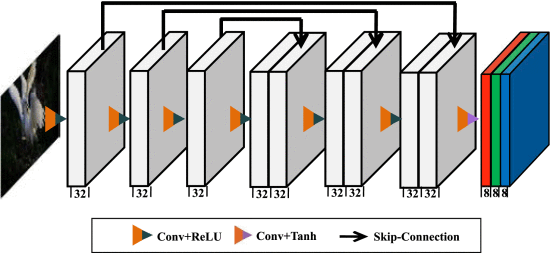
\includegraphics[width=0.8\linewidth]{images/dce-net.png}
    \caption{The architecture of DCE-Net.}
    \label{fig:placeholder}
\end{figure}

Our model will use the same network architecture as the DCE-Net. The network is comprised of seven convolutional neural network layers, each applying symmetrical concatenation to keep output the same size as input. The first six layers: 32 convolutional kernels, size 3x3, stride 1, ReLU activation. The last seventh layer: 24 convolutional kernels, size 3x3, stride 1, Tanh activation.

One image passthrough will generate a Light-Enhancement (LE) curve parameter that maps each input pixel brightness to an output pixel brightness in one of the RGB channels. To transform every RGB channel, one pass-through will output three LE curves. After eight iteration passthroughs, the model will have produced a total of eight curves per RGB channel.

Five equations are involved in this neural network, one for mapping input and output, and four for loss and optimization.

\textbf{Equation 1}

The LE curve parameter mapping for a pixel's color channel value:
\[LE(I(x);\alpha)=I(x)+\alpha I(x)(1-I(x))\]
\begin{itemize}
  \item $LE(I(x);\alpha)$ represents the output pixel value for one of the RGB channels
  \item $I(x)$ represents the input pixel value for one of the RGB channels
  \item $\alpha$ represents the trainable parameter affecting the curve magnitude, $\alpha\in[-1,1]$
  \item The idea is that the brighter the input pixel is, the less it will be brightened, while allowing the neural network to decide how much to brighten it by. 
\end{itemize}

\textbf{Equation 2}

The spatial consistency loss:
\begin{equation*} 
L_{spa}=\frac{1}{K}\sum \limits _{i=1}^K\sum \limits _{j\in \Omega (i)}(|(Y_{i}-Y_{j})|-|(I_{i}-I_{j})|)^2, \end{equation*}
\begin{itemize}
  \item $L_{spa}$ represents the loss to optimize
  \item $K$ represents the total number of local regions
  \item $\Omega(i)$ represents the top, right, bottom, and left regions around the $ith$ region
  \item $Y$ represents the average intensity value of the $ith$ region in the enhanced image
  \item $I$ represents the average intensity value of the $ith$ region in the input image
  \item The idea is that the greater the brightness contrast (difference in brightness between pixel regions) within the enhanced image compared to the input image, the greater the loss, so as to preserve brightness contrast.
\end{itemize}

\textbf{Equation 3}

The exposure control loss:
\begin{equation*} 
L_{exp}=\frac{1}{M}\sum \limits _{k=1}^M|Y_{k}-E|, \end{equation*}
\begin{itemize}
  \item $L_{exp}$ represents the loss to optimize
  \item $M$ represents the number of non-overlapping local regions of size 16 × 16
  \item $Y$ represents the average intensity value of the $kth$ local region in the enhanced image
  \item $E$ represents the gray level in RGB
  \item The idea is that the further a region's average color is from gray, the greater the loss, so as to punish under- and over-exposure.
\end{itemize}

\textbf{Equation 4}

The color constancy loss:
\begin{equation*} 
L_{col}=\sum \limits _{\forall (p,q)\in \varepsilon }(J^{p}-J^{q})^2, \varepsilon =\lbrace (R,G),(R,B),(G,B)\rbrace, \end{equation*}
\begin{itemize}
  \item $L_{col}$ represents the loss to optimize
  \item $\epsilon$ represents every pair in RGB
  \item $J^p$ represents the average intensity value of the enhanced image for the $pth$ color channel
  \item $J^q$ represents the average intensity value of the enhanced image for the $qth$ color channel
  \item The idea is that the greater the average difference is between color channels in the enhanced image, the greater the loss, so as to prevent color distortion.
\end{itemize}

\textbf{Equation 5}

The illumination smoothness loss:
\begin{equation*} 
L_{tv_\mathcal {A}}=\frac{1}{N}\sum \limits _{n=1}^N\sum \limits _{c\in \xi }(|\nabla _{x}\mathcal {A}_{n}^{c}|+|\nabla _{y}\mathcal {A}_{n}^{c}|)^2, \xi =\lbrace R,G,B\rbrace, \end{equation*}
\begin{itemize}
  \item $L_{tv_\mathcal {A}}$ represents the loss to optimize
  \item $N$ represents the number of iterations
  \item $\xi$ represents the three color channels
  \item $\nabla _{x}$ represents the horizontal brightness gradient
  \item $A$ represents a color channel's LE curve parameter mapping
  \item $\nabla _{y}$ represents the vertical brightness gradient
  \item The idea is that the greater and more frequent there are jumps in neighboring pixel intensities, the greater the loss, so as to reflect the gradual shifts in brightness in reality.
\end{itemize}

\textbf{Zero-DCE++}

In the Zero-DCE++, the first six layers: depthwise convolution, kernels size 3×3, stride 1, ReLU activation. The last seventh layer: pointwise convolution, kernels size 1×1, stride 1, Tanh activation. The same 3 LE curve parameter mappings are reused across 8 iterations. The input is downsampled by a factor of 12 before computing the LE curves with the assumption that each curve can be upsampled to generalize and map to a pixel region on the output image because pixels within the same region tend to share similar intensity.

\subsection{Training Setup}

\begin{tabular}{|l|p{12.5cm}|}
\toprule
\textbf{Hyperparameter} & \textbf{Value} \\
\midrule
Optimiser & Adam \\
Learning rate & $1\times{10}^{-4}$ \\
Weight decay & $1\times{10}^{-4}$ \\
Gradient clip norm & $1\times{10}^{-1}$ \\
Epochs / iterations & 200 \\
Batch size & 8 \\
Loss function & spatial consistency loss (weight 1), exposure control loss (weight 1), color constancy loss (weight 0.5), and illumination smoothness loss (weight 20) \\
Random seeds used & 42, 123, 999 \\
\bottomrule
\end{tabular}

\subsection{Dataset and Preprocessing}

The datasets we will use for baseline reproduction is the Single Image Contrast Enhancement (SICE) dataset's part 1 and 2 subsets for training and testing respectively, which was how Zero-DCE was evaluated for Peak-Signal-To-Use Ratio (PSNR) and Structural Similarity Index Measure (SSIM) in the published paper.

All of the images were resized to 1200 (width) x 900 (height) x 3 (RGB channels). The testing set contained sequences, each of the same image in different brightnesses. Filtering the testing set was, as in the paper, as follows:

\begin{itemize}
    \item If a sequence has 7 images, take the darkest 3
    \item If a sequence has 9 images, take the darkest 4
\end{itemize}

The filtering rule for sequences with 5, 6, or 8 images wasn't mentioned in the paper, so our best estimation of their approach is as follows:

\begin{itemize}
    \item If a sequence has 5 or 6 images, take the darkest 2
    \item If a sequence has 8 images, take the darkest 3
\end{itemize}

As such, the training set has 3021 samples and the testing set has 767 (matching the paper) samples, for a train-set split of 80:20.

The inference algorithm for Zero-DCE performs two preprocessing steps: \\
1. Pixel value normalization: transform pixel values to range between 0 and 1, happens during training and testing \\
2. Resizing: transform input into uniform sizes to allow batching, happens only during training

\section{Preliminary Results}

\subsection{Baseline Reproduction}

\begin{center}
\begin{tabular}{lcc}
\toprule
\textbf{Model} & \textbf{PSNR (Mean $\pm$ Std)} & \textbf{SSIM (Mean $\pm$ Std)} \\
\midrule
Published Zero-DCE & 16.57 & 0.59 \\
Published Zero-DCE++ & 16.42 & 0.58 \\
Reproduced Zero-DCE & 12.22 $\pm$ 1.51 & 0.46 $\pm$ 0.15 \\
Reproduced Zero-DCE++ & 9.50 $\pm$ 0.97 & 0.46 $\pm$ 0.15 \\
\bottomrule
\end{tabular}
\captionof{table}{Preliminary results trained on the SICE dataset Part 1 subset and tested on the Part 2 subset. A 80:20 train-test split. All results are mean $\pm$ std over 5 seeds.}
\end{center}

\subsection{Qualitative Analysis}

\begin{figure}[H]
  \centering
  
  % "Before" Image
  \begin{subfigure}{0.40\textwidth}
    \centering
    
\includegraphics[width=\linewidth]{images/trooper-before.png}
    \caption{Input}
    \label{fig:before}
  \end{subfigure}
  \hfill % Adds horizontal space and pushes the images to the edges
  % "After" Image
  \begin{subfigure}{0.40\textwidth}
    \centering
    
\includegraphics[width=\linewidth]{images/trooper-after.png}
    \caption{Enhanced by published Zero-DCE}
    \label{fig:after}
  \end{subfigure}
  % "After" Image
  \begin{subfigure}{0.40\textwidth}
    \centering
    
\includegraphics[width=\linewidth]{images/trooper-after-extension.png}
    \caption{Enhanced by published Zero-DCE++}
    \label{fig:after}
  \end{subfigure}

  \caption{Testing the published Zero-DCE and Zero-DCE++ on one of the test images in the published repository to check its performance on extremely dark images.}
  \label{fig:comparison}
\end{figure}

\begin{figure}[H]
  \centering
  
  % "Before" Image
  \begin{subfigure}{0.49\textwidth}
    \centering
    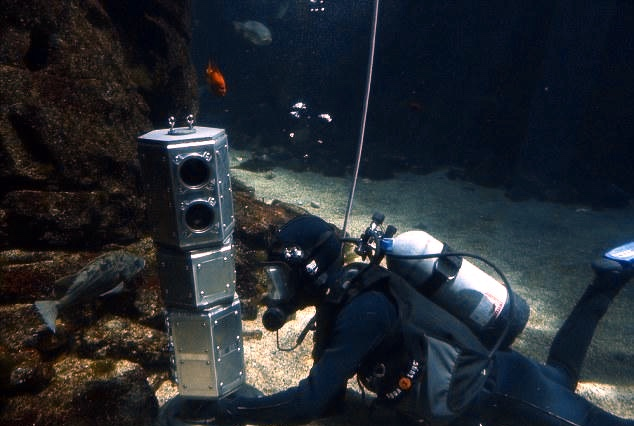
\includegraphics[width=\linewidth]{images/underwater-before.png}
    \caption{Input from the UIEB dataset}
    \label{fig:before}
  \end{subfigure}
  \hfill % Adds horizontal space and pushes the images to the edges
  % "After" Image
  \begin{subfigure}{0.49\textwidth}
    \centering
    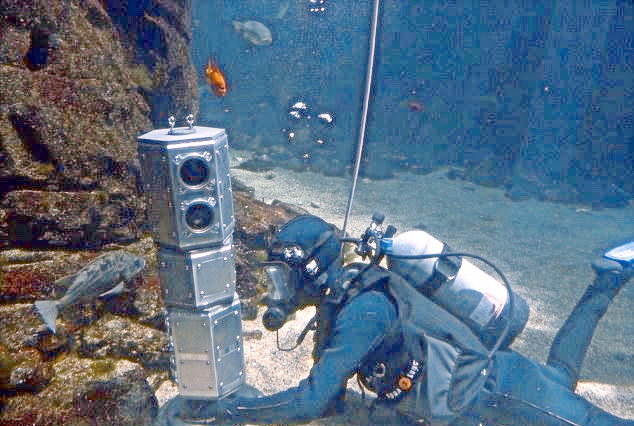
\includegraphics[width=\linewidth]{images/underwater-after.png}
    \caption{Enhanced by published Zero-DCE}
    \label{fig:after}
  \end{subfigure}
  % "After" Image
  \begin{subfigure}{0.49\textwidth}
    \centering
    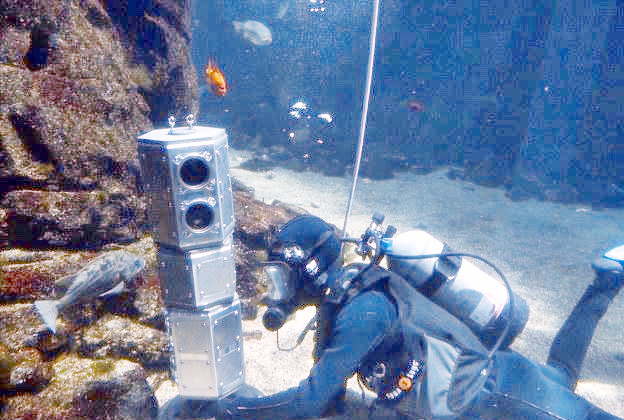
\includegraphics[width=\linewidth]{images/underwater-after-extension.png}
    \caption{Enhanced by published Zero-DCE++}
    \label{fig:after}
  \end{subfigure}

  \caption{Testing the published Zero-DCE and Zero-DCE++ on the 400th image in the UIEB dataset to check its performance in the underwater domain.}
  \label{fig:comparison}
\end{figure}

\subsection{Discussion}

Figure 2 shows an example where Zero-DCE's performance degrades and outputs with a significant, unnatural purple tint. We believe the cause lies in the dark regions being extremely dark with an initial bias toward purple. Upon checking a pixel in the input image's dark regions, the RGB values found were 16, 4, and 18 respectively, showing definitive bias toward purple. It may explain why the purple tint is so obstinate in the output despite the effect of a color constancy loss to punish color deviation. The enhancement process would iteratively scale these RGB values, which would also scale the proportional difference between color channels, retaining the purple bias in the output.

In figure 3, Zero-DCE and Zero-DCE++ visibly improved the brightness in the image at the cost of significantly amplifying noise. This aligns with our existing hypothesis that the model's current approach to enhancement is ill-suited for handling the visual pollution in underwater environments. One of our proposed extensions introduces the use of a denoiser which may help mitigate this issue.

Zero-DCE and Zero-DCE++ for the most part produce the same output, and Zero-DCE++ as expected has proven to be much quicker in training and testing.

\section{Challenges and Adaptations}

One technical issue we ran into was that there were greater hardware specifications than expected to run the published Zero-DCE. Inference on images already resized for training would take seconds to minutes on an Intel i5 CPU. At this rate, training would have taken days straight, and so the decision was made to move testing onto Google Colab and their GPUs.

There were numerous issues trying to use the repository provided by the paper. For example, code not running due to inconsistent formatting, data with file type ".JPG" not loading during training due to a ".jpg" search expression, and hardcoded randomization seeds. We've added fixes and updates to resolve these issues.

Our reproduced metrics have fallen short of the ones published in the paper. The cause may be differences in the exact hyperparameters used by the repository model and the one in the paper. For example, the number of epochs were not mentioned and are unclear. We will try resolving this issue by experimenting with different hyperparameter value and ensuring the model matches the descriptions in the paper.

\section{Project Timeline and Roles}

\begin{center}
\begin{tabular}{lp{7cm}l}
\toprule
\textbf{Week} & \textbf{Tasks} & \textbf{Responsible} \\
\midrule
7 & Run user study, test on UIEB dataset. & Andrew, Ray \\
8 & Run ablation studies, calculate metrics. & Ray \\
9 & Create visual grids, clean code, draft final report. & Andrew, Snowman \\
10 & Finalize report, prepare presentation. \textbf{(Final due)} & All \\
\bottomrule
\end{tabular}
\end{center}

\subsection{Contribution Declaration}

\begin{tabular}{lcc}
\toprule
\textbf{Member} & \textbf{Primary Responsibilities} & \textbf{Estimated \%} \\
\midrule
Andrew Oh & Project management, report writing. & 33.3\%  \\
Ray Shi & Literature review, metrics evaluation, ablation studies. & 33.3\%  \\
Abominable Snowman & Model coding, baseline reproduction, GitHub management. & 33.3\%  \\
\bottomrule
\end{tabular}

\section{References}

\begin{enumerate}[label={[\arabic*]},leftmargin=*]
  \item Guo et al, Year. ``Zero-Reference Deep Curve Estimation for Low-Light Image Enhancement.'' \textit{CVPR}. arXiv:2001.06826.
  \item Li et al, 2021. ``Learning to Enhance Low-Light Image via Zero-Reference Deep Curve Estimation..'' \textit{TPAMI}. arXiv:2207.08789.
  \item Xu et al, 2022. ``SNR-Aware Low-Light Image Enhancement..'' \textit{CVPR}. rXiv:1901.05495.
  \item Zamir et al, 2020., 2020. ``Learning Enriched Features for Real Image Restoration and Enhancement.'' \textit{ECCV}. arXiv:2003.06792.
  \item Li et al, 2019, ``An Underwater Image Enhancement Benchmark Dataset and Beyond.'' \textit{IEEE}. arXiv:1901.05495.
  \item Islam et al, 2020,``Fast Underwater Image Enhancement for Improved Visual Perception.'' \textit{IEEE}. arXiv:2003.11411.
\end{enumerate}

\end{document}